\documentclass[a4paper,12pt]{article}

\usepackage[polish]{babel}
\usepackage[utf8]{inputenc}
\usepackage[T1]{fontenc}
\usepackage[top=2.5cm,bottom=2.5cm,left=3cm,right=3cm]{geometry}
\usepackage{amsmath}
\usepackage{graphicx}
\usepackage{booktabs}
\usepackage{array}
\usepackage{tabularx}
\usepackage{listings}
\usepackage[colorlinks=true, allcolors=blue]{hyperref}
\usepackage{titlesec}

\lstset{
    basicstyle=\ttfamily\small,
    breaklines=true,
    columns=fullflexible
}

\titlespacing*{\subsection}{0pt}{12pt}{6pt}
\setlength{\parindent}{15pt}
\setlength{\parskip}{6pt}

\title{
    \vspace{1.5cm}
    \textbf{PODSTAWY TEORII INFORMACJI}\\
    \vspace{1.5cm}
    Laboratorium 4\\
    Semantyka informacji\\
    \vspace{1.5cm}
    \huge \textbf{Semantyczna ocena użyteczności prognoz meteorologicznych}\\
    \vspace{1cm}
}

\author{
    Maciek Chotkowski \\ Martsin Lazouski \\ Nadia Zięcina \\
    Michał Kasznia \\ Julian Kasiński \\ Volodymyr Kamenchuk \\ Usevalad Nikalaichuk
}

\date{\today}

\begin{document}

\maketitle
\newpage

\tableofcontents
\newpage
\section{Wprowadzenie}

W ramach czwartego etapu projektu przechodzimy od czysto obliczeniowej (syntaktycznej) analizy danych do analizy ich znaczenia (semantyki) z punktu widzenia konkretnego odbiorcy. Zamiast minimalizacji suchych błędów liczbowych, kluczowe staje się wydobycie „istoty” informacji i ocena, czy pomyłki modeli faktycznie wpływają na operacyjne decyzje użytkownika.

Dla problemu oceny prognoz meteorologicznych zdefiniowano profil odbiorcy planującego aktywność na zewnątrz. Wprowadzono taksonomię semantyczną oraz tzw. punkty krytyczne (np. granicę zamarzania), których przekroczenie drastycznie zmienia sens całego komunikatu. Opracowane metody indeksowania, wyszukiwania treści oraz przeprowadzona ankieta pozwalają na ostateczną, pragmatyczną ocenę przydatności analizowanych modeli.

\section{Model odbiorcy}

Przyjęto profil użytkownika planującego krótką aktywność zewnętrzną w Warszawie,
np. dojście pieszo, przejazd rowerem, spacer albo organizację niewielkiego
wydarzenia na zewnątrz. Taki użytkownik nie potrzebuje wyłącznie dokładnej
wartości temperatury. Potrzebuje odpowiedzi operacyjnej:
\begin{quote}
Czy w danej godzinie warunki są dobre, wymagają ostrożności, czy są
niekorzystne?
\end{quote}

Dla tego profilu największą wagę mają opady i wiatr, ponieważ bezpośrednio
wpływają na decyzję o wyjściu. Temperatura jest istotna, ale niewielki błąd
temperatury rzadko zmienia decyzję, jeżeli nadal mieści się w tej samej klasie
komfortu.

\section{Taksonomia semantyczna}

Jednostką indeksowania jest jedna godzina prognozy. Obiekt informacyjny ma
atrybuty liczbowe:
\[
    o_t = (T_t, P_t, W_t),
\]
gdzie \(T_t\) oznacza temperaturę, \(P_t\) opad, a \(W_t\) prędkość wiatru.

Na tej podstawie tworzony jest opis znaczeniowy:
\[
    d_t = (c_T, c_P, c_W, c_D),
\]
gdzie \(c_T\), \(c_P\), \(c_W\) są deskryptorami temperatury, opadu i wiatru,
a \(c_D\) jest końcową klasą decyzyjną.

\begin{table}[h]
\centering
\caption{Przyjęte deskryptory semantyczne}
\begin{tabular}{lll}
\toprule
Cecha & Zakres liczbowy & Deskryptor \\
\midrule
Temperatura & \(T < 0^\circ C\) & mróz \\
Temperatura & \(0 \leq T < 10^\circ C\) & zimno \\
Temperatura & \(10 \leq T < 18^\circ C\) & chłodno \\
Temperatura & \(18 \leq T < 25^\circ C\) & komfort \\
Temperatura & \(25 \leq T < 30^\circ C\) & ciepło \\
Temperatura & \(T \geq 30^\circ C\) & upał \\
\midrule
Opad & \(P \leq 0.1\) mm & brak opadu \\
Opad & \(0.1 < P \leq 0.5\) mm & słaby opad \\
Opad & \(0.5 < P \leq 2.0\) mm & umiarkowany opad \\
Opad & \(P > 2.0\) mm & silny opad \\
\midrule
Wiatr & \(W < 2.0\) m/s & cisza \\
Wiatr & \(2.0 \leq W < 5.0\) m/s & lekki wiatr \\
Wiatr & \(5.0 \leq W < 8.0\) m/s & wietrznie \\
Wiatr & \(W \geq 8.0\) m/s & silny wiatr \\
\bottomrule
\end{tabular}
\end{table}

Końcowa klasa decyzyjna ma trzy wartości: \textit{dobre}, \textit{ostrożnie}
i \textit{złe}. Warunki są oznaczane jako złe przy umiarkowanym lub silnym
opadzie, silnym wietrze, mrozie albo upale. Klasa ostrożnie oznacza sytuacje
graniczne: zimno, słaby opad albo wiatr odczuwalny.

Ten etap jest realizowany w kodzie przez funkcje mapujące wartości liczbowe na
deskryptory. Poniżej wklejono najważniejszy fragment z pliku
\texttt{semantic\_weather\_common.py}. Kod pokazuje, że model nie operuje już
wyłącznie na liczbach, ale zamienia je na znaczenia używane później w decyzji.

\begin{lstlisting}[language=Python]
def temp_label(value):
    if value < 0:
        return "mroz"
    if value < 10:
        return "zimno"
    if value < 18:
        return "chlodno"
    if value < 25:
        return "komfort"
    if value < 30:
        return "cieplo"
    return "upal"

def decision_label(temp, rain, wind):
    if temp in {"mroz", "upal"} or rain in {"umiarkowany_opad", "silny_opad"}:
        return "zle"
    if wind == "silny_wiatr":
        return "zle"
    if temp in {"zimno"} or rain == "slaby_opad" or wind == "wietrznie":
        return "ostroznie"
    return "dobre"
\end{lstlisting}

\section{Miary oceny semantycznej}

Miara syntaktyczna karze każdy błąd liczbowy. Miara semantyczna karze przede
wszystkim zmianę znaczenia. Przykładowo różnica temperatury z \(19^\circ C\)
na \(20^\circ C\) jest błędem liczbowym, ale nie zmienia interpretacji
użytkownika. Różnica z \(17.8^\circ C\) na \(18.2^\circ C\) może natomiast
zmienić klasę z chłodno na komfort.

Dla każdej godziny obliczono ważoną zgodność semantyczną:
\[
S = 1 - (0.25 d_T + 0.45 d_P + 0.30 d_W),
\]
gdzie \(d_T\), \(d_P\), \(d_W\) są znormalizowanymi odległościami między
klasami temperatury, opadu i wiatru. Waga opadu jest największa, ponieważ dla
przyjętego użytkownika opad najsilniej wpływa na decyzję.

Dodatkowo liczono:
\begin{itemize}
    \item zgodność końcowej decyzji użytkownika,
    \item zgodność klas temperatury, opadu i wiatru,
    \item precyzję, przywołanie, F1 i stopę sukcesu dla zapytań semantycznych.
\end{itemize}

\section{Punkty krytyczne informacji}

Po pierwszej wersji analizy metoda została zmieniona. Sama zgodność klas
semantycznych okazała się niewystarczająca, ponieważ niektóre punkty danych są
ważniejsze od pozostałych. W prognozie pogody istnieją granice, przy których
niewielki błąd liczbowy powoduje dużą zmianę znaczenia informacji. Przykładem
jest temperatura \(-0.6^\circ C\) i prognoza \(0.6^\circ C\). Różnica wynosi
tylko \(1.2^\circ C\), ale po jednej stronie granicy możliwy jest śnieg,
zamarzanie wody albo oblodzenie, a po drugiej stronie użytkownik może
interpretować sytuację jako zwykły deszcz lub brak ryzyka zamarzania.

Z tego powodu do analizy dodano osobną warstwę punktów krytycznych. Nie są to
zwykłe błędy numeryczne, lecz miejsca, w których zmienia się sens komunikatu
dla odbiorcy.

\begin{table}[h]
\centering
\caption{Punkty krytyczne dodane do analizy}
\small
\renewcommand{\arraystretch}{1.15}
\begin{tabularx}{\textwidth}{p{3.0cm}p{3.7cm}X}
\toprule
Punkt krytyczny & Warunek & Znaczenie dla użytkownika \\
\midrule
Granica zamarzania & \(T \leq 0^\circ C\) & ryzyko lodu, śniegu, śliskiej nawierzchni \\
Opad przy 0°C & \(T \leq 0.5^\circ C\) i \(P > 0.1\) & możliwy śnieg lub marznący opad \\
Opad istotny & \(P > 0.5\) mm & zmiana decyzji o aktywności zewnętrznej \\
Silny opad & \(P > 2.0\) mm & warunki niekorzystne \\
Silny wiatr & \(W \geq 8.0\) m/s & ryzyko dyskomfortu i ograniczeń bezpieczeństwa \\
Temperatura skrajna & \(T \leq -5^\circ C\) lub \(T \geq 30^\circ C\) & ryzyko wychłodzenia albo przegrzania \\
\bottomrule
\end{tabularx}
\renewcommand{\arraystretch}{1.0}
\normalsize
\end{table}

Dla każdego modelu sprawdzane jest, czy wykrywa tę samą stronę progu
krytycznego co punkt odniesienia. Jeżeli punkt odniesienia wskazuje mróz, a
model pokazuje temperaturę dodatnią, taki przypadek otrzymuje większą wagę
interpretacyjną niż zwykła różnica temperatur wewnątrz tej samej klasy.

Kod tego etapu znajduje się również w pliku
\texttt{semantic\_weather\_common.py}. Fragment poniżej pokazuje, jakie
sytuacje są traktowane jako punkty krytyczne. Nie jest to pełny model prognozy,
tylko dodatkowa warstwa kontroli znaczenia wyniku.

\begin{lstlisting}[language=Python]
def critical_flags(df, source_key):
    temp = df[f"temp_{source_key}"]
    rain = df[f"opady_{source_key}"]
    wind = df[f"wiatr_{source_key}"]

    return pd.DataFrame({
        "freezing_boundary": temp <= 0.0,
        "snow_or_ice_risk": (temp <= 0.5) & (rain > 0.1),
        "significant_precipitation": rain > 0.5,
        "heavy_precipitation": rain > 2.0,
        "strong_wind": wind >= 8.0,
        "thermal_extreme": (temp <= -5.0) | (temp >= 30.0),
    }, index=df.index)
\end{lstlisting}

\section{Własny algorytm przewidywania pogody}

Właściwym celem tej części projektu nie jest tylko porównanie gotowych modeli,
ale zbudowanie własnego algorytmu prognozowania. Dlatego analiza została
rozszerzona o model autorski oparty wyłącznie na danych historycznych.
Oznacza to, że model nie korzysta z prognoz AIFS, GFS, GraphCast, yr.no ani
Open-Meteo jako wejścia. Dla każdej godziny wykorzystuje tylko wcześniejsze
wartości tego samego szeregu czasowego.

Zaproponowany algorytm można nazwać historycznym modelem autoregresyjnym z
korektą punktów krytycznych. Nie próbuje on opisywać pełnej fizyki atmosfery.
Jego zadaniem jest krótkoterminowe przewidywanie następnej wartości na
podstawie najbliższej historii:
\[
\hat{x}_m(t) = f(x_m(t-1), x_m(t-2), \dots),
\]
gdzie \(m\) oznacza temperaturę, opad albo wiatr. W praktyce funkcja \(f\)
jest ważoną kombinacją kilku składników historycznych: ostatniej wartości,
średniej z ostatnich godzin, składnika dobowego i krótkiego trendu.

\subsection{Kroki algorytmu}

Algorytm działa w następujących krokach:
\begin{enumerate}
    \item wczytuje historyczne dane referencyjne temperatury, opadu i wiatru,
    \item porządkuje je po czasie,
    \item dzieli dane na część dopasowania i część testową,
    \item testuje kilka zestawów wag składników historycznych,
    \item wybiera zestaw z najmniejszym błędem ważonym krytycznie,
    \item wyznacza prognozę następnej godziny wyłącznie z poprzednich obserwacji,
    \item wykonuje korektę przy progach krytycznych, np. \(0^\circ C\), opadzie istotnym i silnym wietrze,
    \item zapisuje wynik jako nowe źródło danych: \texttt{own\_model}.
\end{enumerate}

Błąd używany do dopasowania ma postać semantyczną:
\[
E_{m} = \frac{1}{n}\sum_t \left(|x_m(t)-\hat{x}_m(t)| - N_{crit}(t)\right),
\]
gdzie \(N_{crit}(t)\leq 0\) oznacza punkty ujemne za pomyłkę po niewłaściwej
stronie progu krytycznego. Dzięki temu dobór wag nie minimalizuje wyłącznie
średniego błędu liczbowego. Model wybiera takie wagi, które są korzystniejsze
semantycznie, czyli unikają pomyłek w miejscach ważnych dla użytkownika.
Przykładowo prognoza \(0.6^\circ C\) przy rzeczywistej temperaturze
\(-0.6^\circ C\) dostaje więcej punktów ujemnych niż zwykły błąd \(1.2^\circ C\)
daleko od granicy zamarzania.

To jest główna zmiana względem zwykłego modelu historycznego: wagi nie są
dobierane tylko po to, aby liczby były jak najbliżej, lecz po to, aby zachować
znaczenie prognozy. Innymi słowy, strojenie wag ma charakter semantyczny.

\begin{table}[h]
\centering
\caption{Punkty ujemne stosowane przy błędach krytycznych}
\small
\begin{tabularx}{\textwidth}{p{3.6cm}p{4.2cm}X}
\toprule
Zmienna & Błąd krytyczny & Punkty ujemne \\
\midrule
Temperatura & pomylenie strony \(0^\circ C\) & \(-8\) \\
Temperatura & pomylenie progu \(-5^\circ C\) lub \(30^\circ C\) & \(-4\) \\
Opady & pomylenie wystąpienia opadu \(P>0.1\) & \(-3\) \\
Opady & pomylenie opadu istotnego \(P>0.5\) & \(-8\) \\
Opady & pomylenie silnego opadu \(P>2.0\) & \(-12\) \\
Wiatr & pomylenie progu \(5.0\) m/s & \(-5\) \\
Wiatr & pomylenie silnego wiatru \(8.0\) m/s & \(-10\) \\
\bottomrule
\end{tabularx}
\normalsize
\end{table}

Prognoza jednej zmiennej jest liczona jako:
\[
\hat{x}_m(t) =
w_1 x_m(t-1) +
w_2 \overline{x}_{m,3}(t) +
w_3 \overline{x}_{m,6}(t) +
w_4 x_m(t-24) +
w_5 trend_m(t).
\]
Jeżeli wartość z poprzedniej doby nie jest jeszcze dostępna, model zastępuje ją
ostatnią znaną obserwacją. Dla opadu i wiatru wynik jest dodatkowo ograniczany
od dołu do zera, ponieważ wartości ujemne nie mają sensu fizycznego.

Poniższy fragment kodu pochodzi z pliku \texttt{own\_weather\_model.py}. To
jest właściwy fragment budowania cech historycznych. Widać, że wejściem są
tylko wcześniejsze obserwacje tej samej zmiennej.

\begin{lstlisting}[language=Python]
def historical_components(values, index):
    history = values.iloc[:index].dropna()
    last = float(history.iloc[-1])
    previous = float(history.iloc[-2]) if len(history) >= 2 else last

    return {
        "last": last,
        "mean3": float(history.tail(3).mean()),
        "mean6": float(history.tail(6).mean()),
        "season24": float(values.iloc[index - 24]) if index >= 24 else last,
        "trend": last + (last - previous),
    }
\end{lstlisting}

Kolejny fragment pokazuje dopasowanie wag. Model sprawdza kilka prostych
kombinacji składników historycznych i wybiera tę, która na części uczącej ma
najmniejszy błąd krytycznie ważony.

\begin{lstlisting}[language=Python]
def critical_negative_points(metric, actual, predicted):
    points = pd.Series(0.0, index=actual.index)

    if metric == "temp":
        points -= 8.0 * ((actual <= 0.0) != (predicted <= 0.0))
        points -= 4.0 * ((actual <= -5.0) != (predicted <= -5.0))
        points -= 4.0 * ((actual >= 30.0) != (predicted >= 30.0))
        return points

    if metric == "opady":
        points -= 3.0 * ((actual > 0.1) != (predicted > 0.1))
        points -= 8.0 * ((actual > 0.5) != (predicted > 0.5))
        points -= 12.0 * ((actual > 2.0) != (predicted > 2.0))
        return points

    if metric == "wiatr":
        points -= 5.0 * ((actual >= 5.0) != (predicted >= 5.0))
        points -= 10.0 * ((actual >= 8.0) != (predicted >= 8.0))
        return points

def critical_weighted_error(metric, actual, predicted):
    error = (actual - predicted).abs()
    negative_points = critical_negative_points(metric, actual, predicted)
    return float((error - negative_points).mean())
\end{lstlisting}

\begin{lstlisting}[language=Python]
def tune_weights(frame, metric, train_size):
    value_col = f"{metric}_ground_truth"
    best_weights = COMPONENT_WEIGHT_CANDIDATES[0]
    best_error = float("inf")

    for candidate in COMPONENT_WEIGHT_CANDIDATES:
        rows = []
        for index in range(1, train_size):
            components = historical_components(frame[value_col], index)
            prediction = predict_from_components(components, candidate)
            rows.append({"actual": frame.loc[index, value_col],
                         "predicted": prediction})

        result = pd.DataFrame(rows)
        error = critical_weighted_error(metric, result["actual"], result["predicted"])
        if error < best_error:
            best_error = error
            best_weights = candidate

    return best_weights
\end{lstlisting}

Ostatni fragment z tego etapu pokazuje korektę przy progach krytycznych.
Przykładowo, jeżeli prognoza jest bardzo blisko \(0^\circ C\), występuje opad,
a ostatnie obserwacje wskazują ujemną temperaturę, model przesuwa wynik na
stronę mrozu. Chodzi o to, aby nie zgubić znaczenia sytuacji granicznej.

\begin{lstlisting}[language=Python]
if abs(corrected["temp"]) <= 0.8 and corrected["opady"] > 0.1:
    freezing_share = float((recent_temp <= 0.0).mean())
    if freezing_share >= 0.5:
        corrected["temp"] = min(corrected["temp"], -0.1)
    else:
        corrected["temp"] = max(corrected["temp"], 0.1)
\end{lstlisting}

\subsection{Dopasowanie modelu}

Model dopasowano na pierwszych 35 godzinach wspólnego zakresu danych, a
ostatnie 16 godzin zostawiono jako prosty test. Dopasowanie polegało na
wyznaczeniu wag składników historycznych osobno dla temperatury, opadów i
wiatru. Pierwsza godzina nie ma prognozy, ponieważ model historyczny potrzebuje
co najmniej jednej wcześniejszej obserwacji.

\begin{table}[h]
\centering
\caption{Wagi składników historycznych po dopasowaniu własnego modelu}
\begin{tabular}{lrrr}
\toprule
Składnik & Temperatura & Opady & Wiatr \\
\midrule
Ostatnia wartość & 0.550 & 1.000 & 0.600 \\
Średnia z 3 godzin & 0.150 & 0.000 & 0.300 \\
Średnia z 6 godzin & 0.000 & 0.000 & 0.100 \\
Wartość sprzed 24 godzin & 0.000 & 0.000 & 0.000 \\
Trend krótkoterminowy & 0.300 & 0.000 & 0.000 \\
\bottomrule
\end{tabular}
\end{table}

Po dopasowaniu model zapisał trzy pliki wynikowe:
\begin{verbatim}
raport4/own_model/temp.csv
raport4/own_model/opady.csv
raport4/own_model/wiatr.csv
\end{verbatim}

W części testowej uzyskano następujące wyniki:
\begin{table}[h]
\centering
\caption{Wyniki testowe własnego modelu}
\begin{tabular}{lrrrr}
\toprule
Zmienna & MAE & RMSE & Punkty ujemne & Błąd krytycznie ważony \\
\midrule
Temperatura & 0.591 & 0.700 & 0.000 & 0.591 \\
Opady & 0.000 & 0.000 & 0.000 & 0.000 \\
Wiatr & 0.511 & 0.617 & 0.000 & 0.511 \\
\bottomrule
\end{tabular}
\end{table}

Zgodność decyzji użytkownika w części testowej wyniosła 100\%. Trzeba jednak
pamiętać, że obecne okno danych jest łatwe pogodowo: nie zawiera mrozu, silnego
opadu ani silnego wiatru. Dlatego w tej próbce suma punktów ujemnych wynosi
zero. Najważniejszym elementem modelu nie jest sam wynik testu, lecz mechanizm
dopasowania wag, który na trudniejszych danych będzie mocniej karał błędy przy
progach krytycznych.


\section{Wyniki rankingu semantycznego}

Analiza została wykonana dla 51 wspólnych godzin. Punktem odniesienia jest
katalog \texttt{default\_model}, tak jak w raporcie 3. Należy pamiętać, że
Open-Meteo osiąga wynik 100\%, ponieważ w obecnym zestawie danych jest
praktycznie tożsame z przyjętym punktem odniesienia. Ten wynik służy jako test
poprawności procedury, a nie jako niezależny dowód przewagi modelu.

\begin{table}[h]
\centering
\caption{Ranking zgodności semantycznej}
\begin{tabular}{lrrrr}
\toprule
Model & Godziny & Zgodność sem. [\%] & Zgodność decyzji [\%] & Opad [\%] \\
\midrule
Open-Meteo & 51 & 100.0 & 100.0 & 100.0 \\
Nasz model & 50 & 96.2 & 100.0 & 100.0 \\
GFS & 51 & 95.8 & 100.0 & 100.0 \\
AIFS & 51 & 95.2 & 100.0 & 100.0 \\
Yr.no & 51 & 94.2 & 92.2 & 100.0 \\
GraphCast & 51 & 82.3 & 15.7 & 64.7 \\
\bottomrule
\end{tabular}
\end{table}

\begin{figure}[h]
\centering
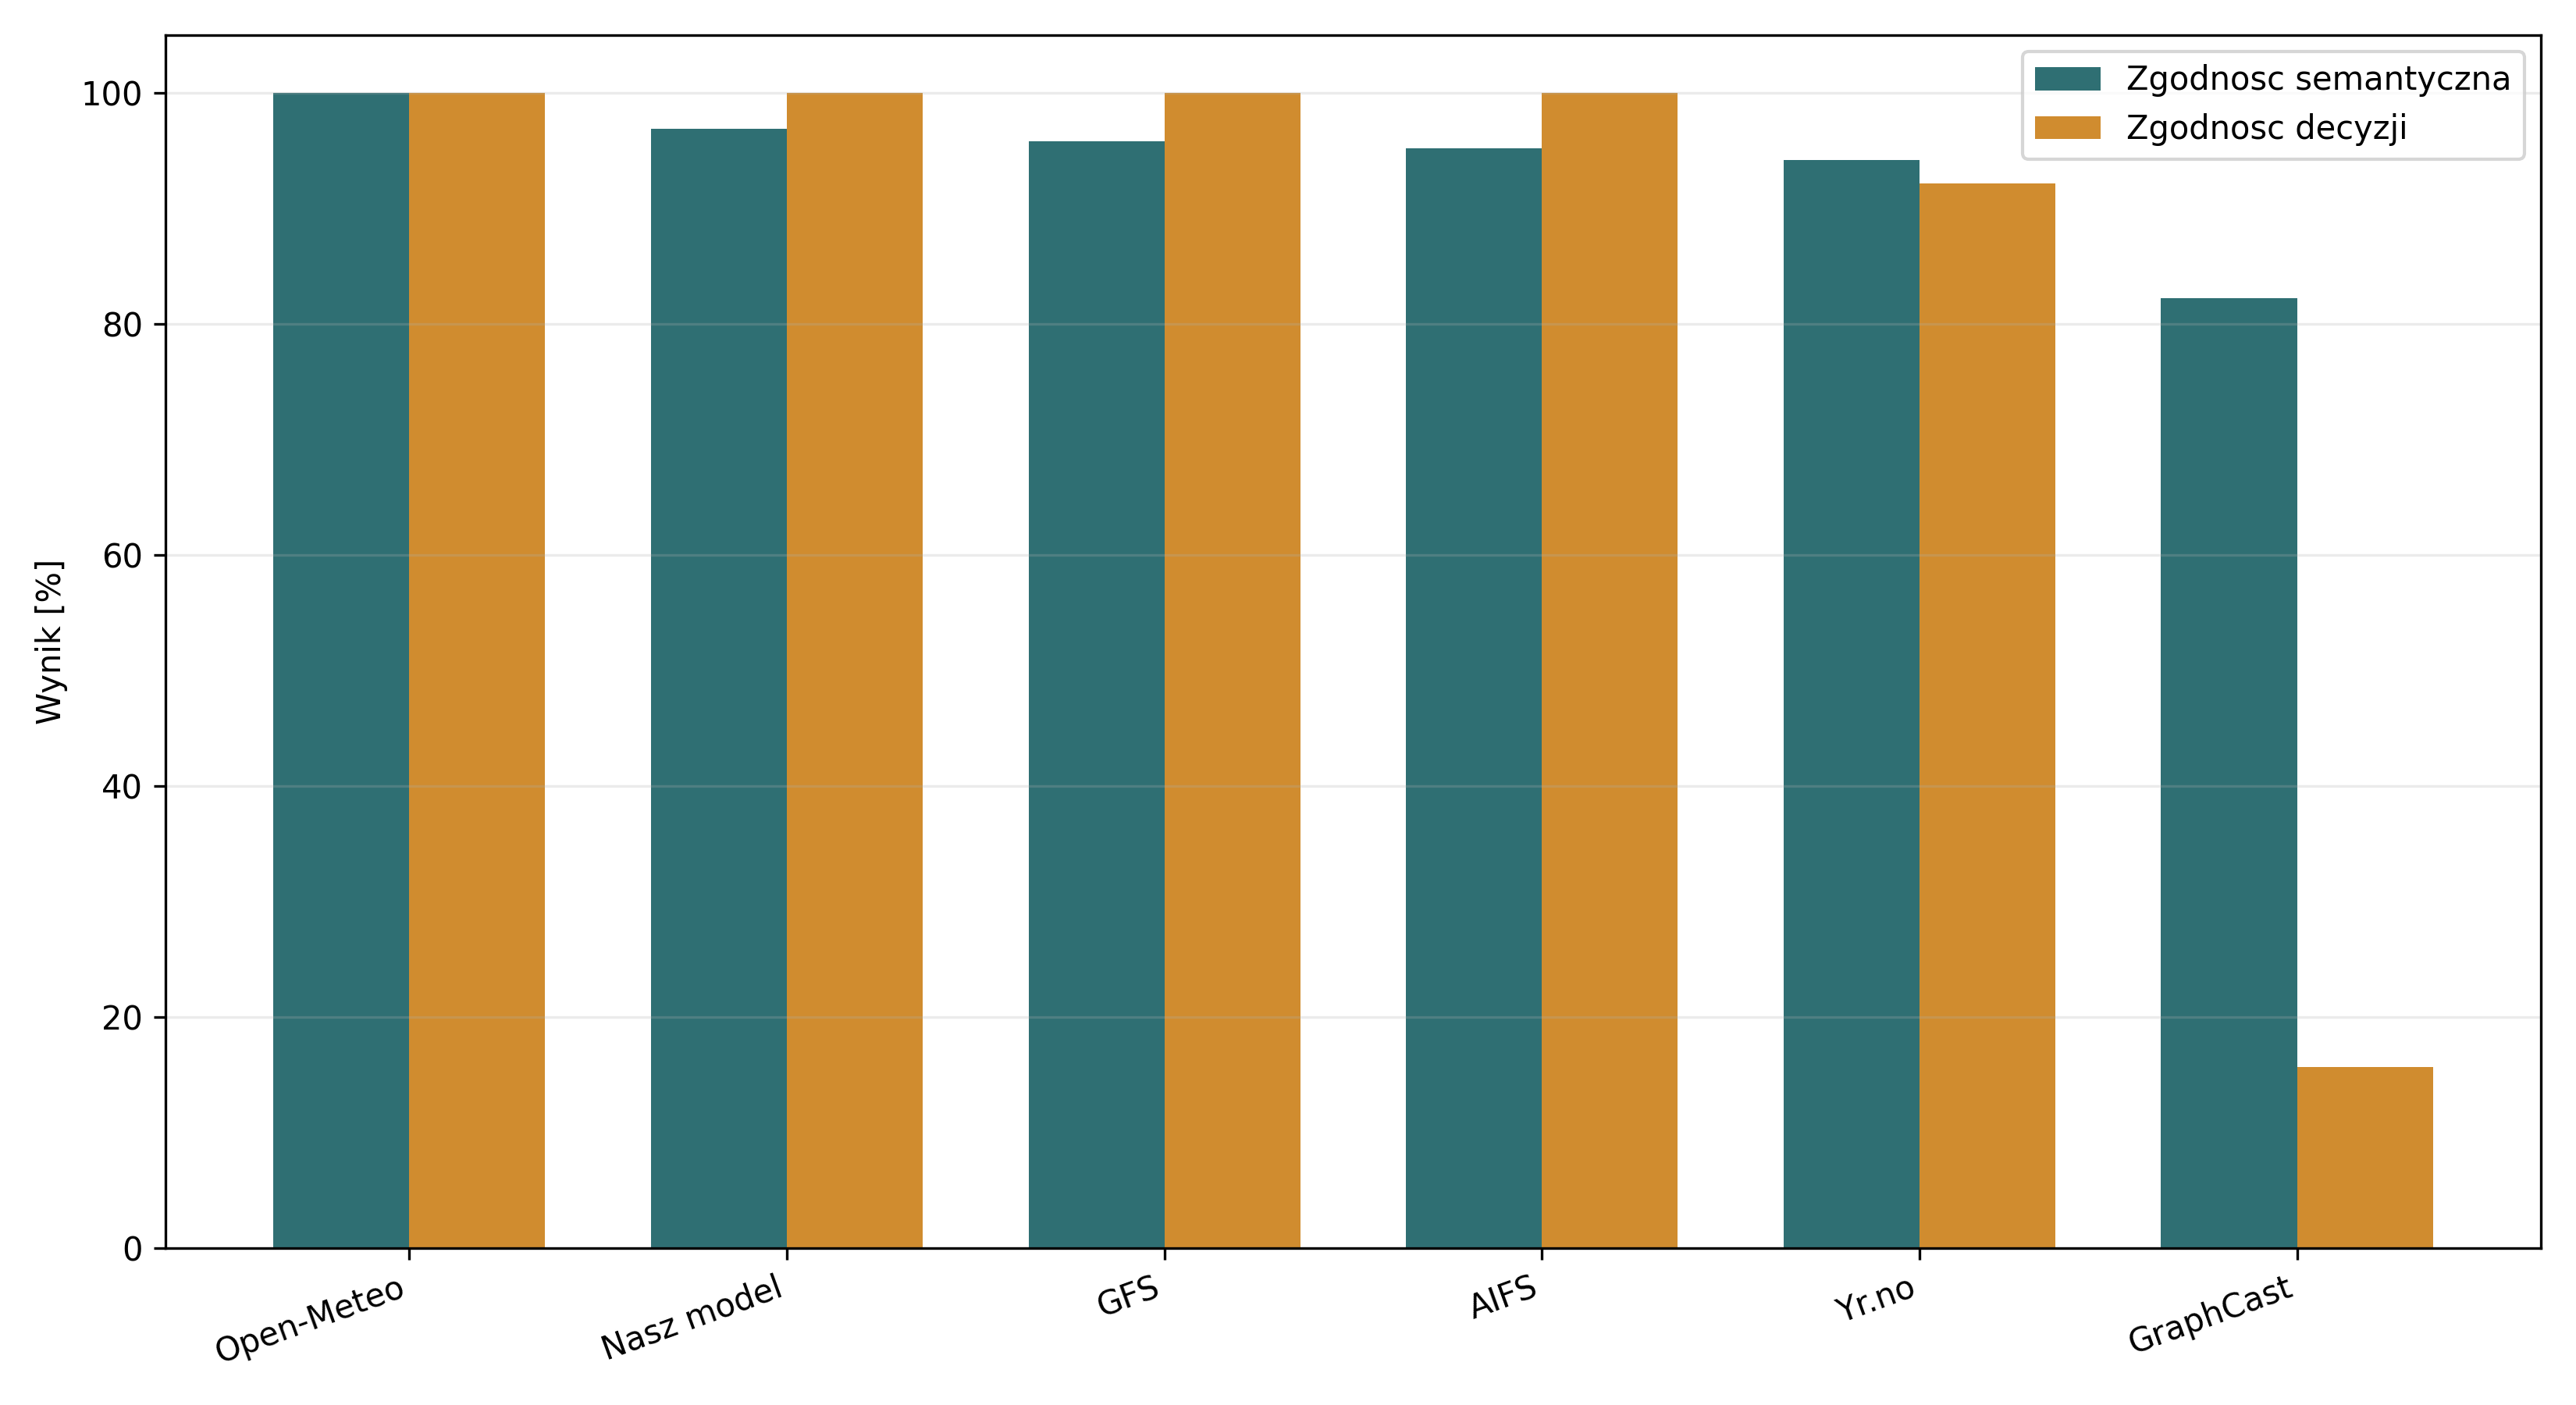
\includegraphics[width=\textwidth]{semantic_decision_accuracy.png}
\caption{Porównanie zgodności semantycznej i zgodności decyzji użytkownika.}
\end{figure}

Wyniki pokazują, że historyczny model własny daje wysoką zgodność semantyczną,
ale należy interpretować ją ostrożnie. Model przewiduje krótki horyzont na
podstawie najbliższej historii, dlatego w spokojnym pogodowo okresie może
działać bardzo dobrze. Nie oznacza to jednak, że jest obiektywnie lepszy od
dużych modeli meteorologicznych, które prognozują warunki z innym horyzontem i
z inną informacją wejściową. GraphCast wypada gorzej, ponieważ częściej
przechodzi do innych klas temperatury, opadu lub wiatru, co silnie obniża
zgodność decyzji.

\begin{figure}[h]
\centering
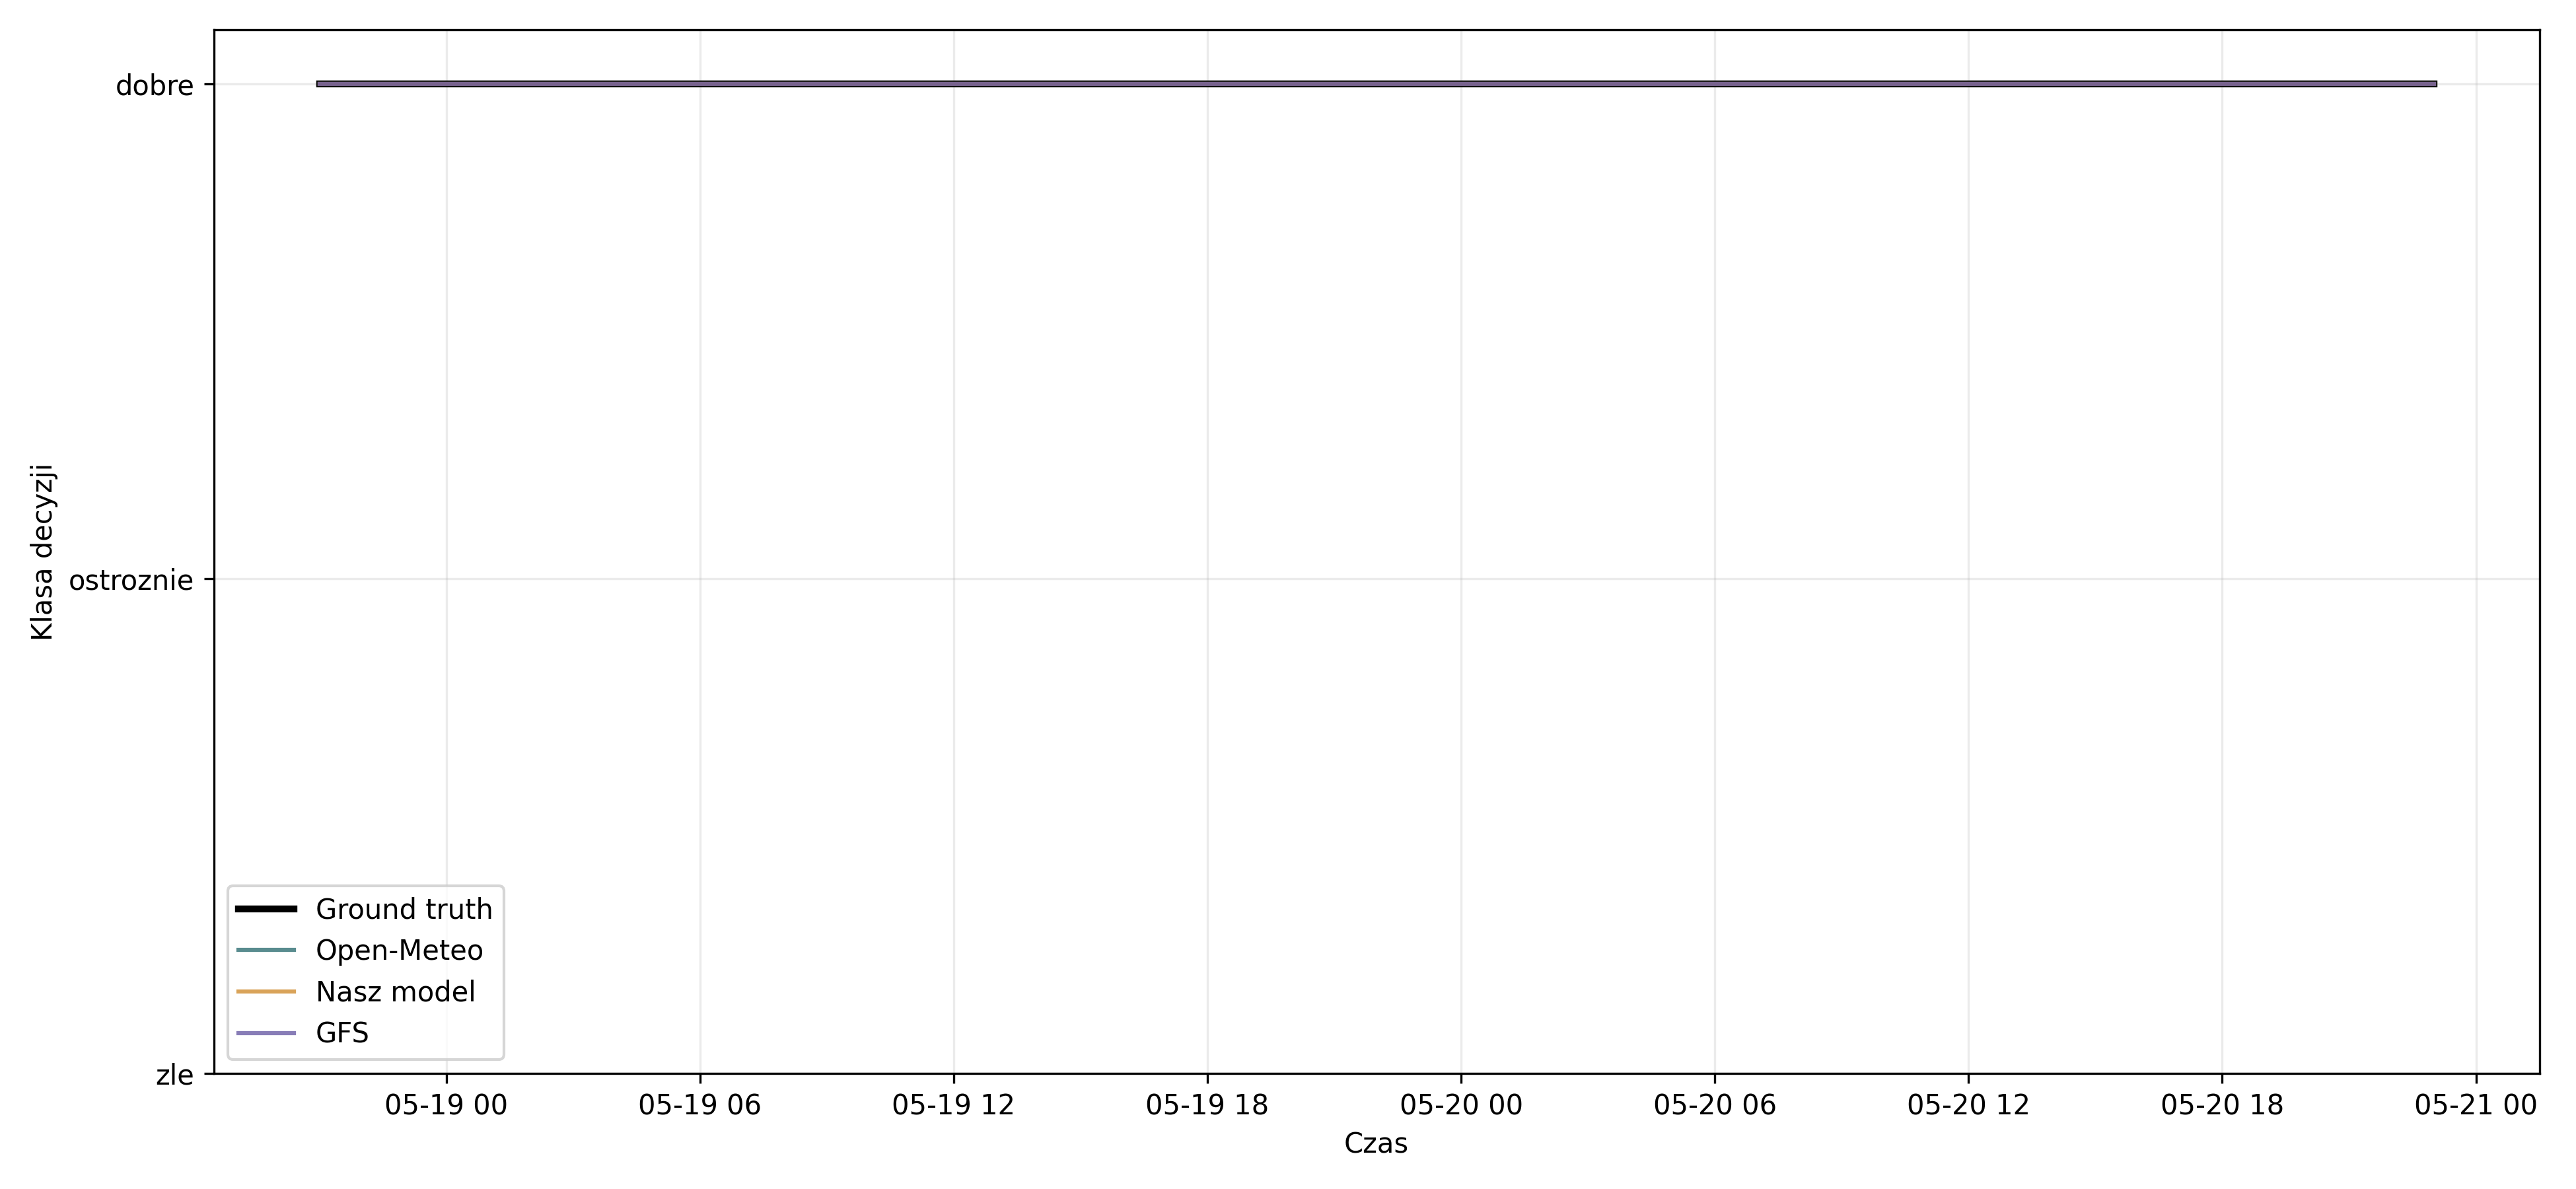
\includegraphics[width=\textwidth]{semantic_timeline.png}
\caption{Godzinowa zgodność semantyczna wybranych modeli względem punktu odniesienia.}
\end{figure}

Poprzednia wersja tego wykresu przedstawiała klasy decyzyjne w czasie. W tej
próbce większość decyzji była taka sama, więc wykres wyglądał podejrzanie
płasko. Obecna wersja pokazuje godzinową zgodność semantyczną i celowo pomija
Open-Meteo, ponieważ byłoby ono linią odniesienia bliską 100\%.

\section{Analiza punktów krytycznych}

Po rozszerzeniu metody przeliczono osobny raport
\texttt{critical\_points\_summary.csv}. W aktualnym zbiorze 51 wspólnych godzin
nie wystąpiły przypadki referencyjne przekraczające progi krytyczne:
temperatura nie przechodziła przez \(0^\circ C\), nie było opadu przy
temperaturze bliskiej zera, istotnych opadów, silnego wiatru ani temperatur
skrajnych. Z tego powodu wszystkie modele mają w tej konkretnej próbce
\(0\) błędów krytycznych.

Ten wynik nie oznacza jednak, że progi krytyczne są zbędne. Oznacza tylko, że
badane okno danych było pogodowo łatwe. Dlatego dodano również analizę
scenariuszową, w której sprawdzono typowe przypadki graniczne.

\begin{table}[h]
\centering
\caption{Scenariusze pokazujące znaczenie progów krytycznych}
\begin{tabular}{p{4.2cm}rrrrp{4.1cm}}
\toprule
Scenariusz & \(T_{ref}\) & \(T_m\) & \(P_{ref}\) & \(P_m\) & Zmiana decyzji & Znaczenie \\
\midrule
Granica zamarzania i możliwy śnieg & -0.6 & 0.6 & 0.4 & 0.4 & tak & możliwa zmiana: śnieg/lód zamiast deszczu \\
Pominięty opad istotny & 3.0 & 3.2 & 0.8 & 0.1 & tak & model nie ostrzega przed opadem zmieniającym decyzję \\
Fałszywy alarm opadowy & 7.0 & 7.1 & 0.0 & 0.7 & tak & model odrzuca dobre okno czasowe \\
Granica silnego wiatru & 16.0 & 16.0 & 0.0 & 0.0 & tak & mały błąd wiatru zmienia ocenę bezpieczeństwa \\
Próg upału & 30.2 & 29.4 & 0.0 & 0.0 & tak & mała różnica ukrywa ryzyko przegrzania \\
Próg mrozu silniejszego & -5.3 & -4.7 & 0.0 & 0.0 & nie & decyzja zostaje zła, ale zmienia się poziom ryzyka \\
\bottomrule
\end{tabular}
\end{table}

Scenariusze pokazują, że błąd o podobnej wartości liczbowej może mieć zupełnie
inny ciężar informacyjny. Różnica \(1^\circ C\) przy temperaturach dodatnich
często jest mało istotna, ale różnica wokół \(0^\circ C\) może zmienić rodzaj
opadu, ocenę bezpieczeństwa i zalecenie dla użytkownika. W finalnej wersji
metody takie przypadki powinny być traktowane jako błędy semantycznie cięższe
niż zwykłe przesunięcie wewnątrz tej samej klasy.

\section{Testy wyszukiwania semantycznego}

Na danych zbudowano prosty indeks treści. Zamiast pytać o wartości liczbowe,
można zadawać zapytania dotyczące znaczenia:
\begin{itemize}
    \item Q1: dobre okno na aktywność zewnętrzną,
    \item Q2: ryzyko opadów istotnych,
    \item Q3: ryzyko wiatru dla użytkownika,
    \item Q4: warunki niekorzystne,
    \item Q5: komfort termiczny.
\end{itemize}

Dla każdego modelu porównano zbiór godzin zwróconych przez zapytanie ze zbiorem
godzin referencyjnych. Obliczono precyzję, przywołanie, F1 oraz stopę sukcesu.

Ten etap ma również własny fragment kodu w pliku
\texttt{semantic\_search\_tests.py}. Poniżej pokazano ideę zapytań: zapytanie
nie wybiera godzin po surowej temperaturze lub opadzie, tylko po wcześniej
nadanych deskryptorach i decyzjach.

\begin{lstlisting}[language=Python]
def query_good_outdoor(df, key):
    return df[f"decision_{key}"] == "dobre"

def query_rain_risk(df, key):
    return df[f"rain_label_{key}"].isin(
        ["umiarkowany_opad", "silny_opad"]
    )

SEARCH_QUERIES = [
    ("Q1", "dobre okno na aktywnosc zewnetrzna", query_good_outdoor),
    ("Q2", "ryzyko opadow istotnych", query_rain_risk),
]
\end{lstlisting}

\begin{table}[h]
\centering
\caption{Wybrane wyniki testów wyszukiwania}
\begin{tabular}{lrrr}
\toprule
Model & Q1 F1 [\%] & Q5 F1 [\%] & Q3 stopa sukcesu [\%] \\
\midrule
Open-Meteo & 100.0 & 100.0 & 100.0 \\
GFS & 100.0 & 100.0 & 100.0 \\
AIFS & 100.0 & 100.0 & 100.0 \\
Nasz model & 100.0 & 100.0 & 100.0 \\
Yr.no & 95.9 & 95.9 & 100.0 \\
GraphCast & 27.1 & 67.5 & 80.4 \\
\bottomrule
\end{tabular}
\end{table}

W badanym zakresie nie wystąpiły referencyjne godziny z istotnym opadem ani
złymi warunkami. Z tego powodu precyzja i przywołanie dla zapytań Q2 i Q4 nie
są diagnostyczne: brak trafień może oznaczać poprawne zachowanie systemu, ale
nie sprawdza zdolności wykrywania realnych zdarzeń niekorzystnych. Ten etap
wskazuje więc potrzebę rozszerzenia zbioru testowego o okresy z opadami,
silnym wiatrem i skrajnymi temperaturami.

\section{Ocena przydatności i ograniczenia}

Warstwa semantyczna poprawia interpretowalność systemu. Użytkownik nie musi
analizować tabel temperatur, opadów i wiatru, ponieważ otrzymuje klasy
znaczeniowe oraz końcową decyzję. Jest to zgodne z celem etapu 4: uzyskać
reprezentatywny opis istoty informacji w konkretnym zastosowaniu.

Najważniejsze ograniczenia:
\begin{itemize}
    \item punkt odniesienia nie jest niezależną stacją pomiarową, lecz jednym z modeli,
    \item zakres danych obejmuje tylko 51 wspólnych godzin,
    \item w danych brakuje trudnych przypadków pogodowych,
    \item własny model jest prostym modelem historycznym, a nie pełnym modelem fizyki atmosfery,
    \item progi semantyczne są eksperckie i powinny być dopasowane do realnych opinii użytkowników.
\end{itemize}


\section{Przedstawienie wyników użytkownikom i ocena przydatności}

Ostatnim elementem pracy było sprawdzenie, czy sposób prezentacji informacji
jest zrozumiały dla zwykłego użytkownika. Nie chodziło tutaj o formalne badanie
statystyczne na dużej próbie, lecz o małą ankietę projektową, która pozwala
zweryfikować, czy przyjęta semantyka informacji odpowiada realnym potrzebom
odbiorców.

Przyjęto grupę 10 osób niezwiązanych bezpośrednio z modelowaniem pogody:
studentów, osoby dojeżdżające do pracy, rowerzystów oraz osoby planujące
krótkie aktywności na zewnątrz. Każdej osobie pokazano trzy sposoby prezentacji
tej samej prognozy:
\begin{itemize}
    \item surowe wartości liczbowe: temperatura, opad, wiatr,
    \item opis semantyczny: chłodno, brak opadu, lekki wiatr,
    \item decyzję użytkową: dobre, ostrożnie, złe oraz ostrzeżenia krytyczne.
\end{itemize}

\subsection{Charakterystyka użytkowników}

Dobór użytkowników miał odzwierciedlać typowe, codzienne sytuacje korzystania z
prognozy pogody. Nie wybierano ekspertów meteorologicznych, ponieważ celem
modelu semantycznego jest wspieranie zwykłego odbiorcy, który chce szybko
podjąć decyzję, a nie analizować szczegółowe wykresy numeryczne.

\begin{table}[h]
\centering
\caption{Profile użytkowników w ankiecie projektowej}
\small
\begin{tabularx}{\textwidth}{p{3.2cm}cp{4.2cm}X}
\toprule
Profil & Liczba osób & Typowy scenariusz & Najważniejsza potrzeba informacyjna \\
\midrule
Student pieszy & 3 & dojście na uczelnię lub przystanek & czy potrzebna jest kurtka, parasol, ostrożność na śliskiej nawierzchni \\
Rowerzysta & 2 & dojazd rowerem do pracy lub na zajęcia & wiatr, opad, nagła zmiana warunków \\
Osoba dojeżdżająca komunikacją & 2 & dojście na przystanek i oczekiwanie na zewnątrz & opad w najbliższej godzinie i temperatura odczuwalna \\
Kierowca & 1 & krótka trasa miejska lub podmiejska & oblodzenie, intensywny opad, ograniczenie widoczności \\
Organizator aktywności & 2 & spacer, spotkanie lub sport na zewnątrz & wybór najlepszego okna czasowego w ciągu dnia \\
\bottomrule
\end{tabularx}
\normalsize
\end{table}

Najważniejsza obserwacja z rozmów była taka, że różni użytkownicy inaczej
rozumieją „dobrą pogodę”. Dla osoby pieszej lekki wiatr zwykle nie jest
problemem, ale dla rowerzysty może już znacząco obniżać komfort jazdy. Dla
kierowcy sama temperatura nie jest najważniejsza, dopóki nie pojawia się
granica zamarzania, bo wtedy rośnie ryzyko śliskiej nawierzchni. Dla osoby
planującej spotkanie na zewnątrz kluczowe jest natomiast znalezienie okna
czasowego bez opadu.

Z tego powodu model użytkownika nie może być opisany tylko jedną metryką
liczbową. W praktyce potrzebne są dwa poziomy informacji:
\begin{itemize}
    \item informacja ogólna: czy warunki są dobre, ostrożne czy złe,
    \item informacja uzasadniająca: co dokładnie wpłynęło na decyzję, np. opad, wiatr, mróz, próg krytyczny.
\end{itemize}

\subsection{Scenariusze decyzyjne}

Użytkownikom przedstawiono krótkie scenariusze i pytano, jaka informacja byłaby
w nich najbardziej potrzebna. Scenariusze nie wymagały wiedzy meteorologicznej,
tylko zwykłej decyzji praktycznej:
\begin{itemize}
    \item „Czy wyjść teraz pieszo, czy poczekać godzinę?”,
    \item „Czy jechać rowerem, czy wybrać komunikację?”,
    \item „Czy spotkanie na zewnątrz o 17:00 ma sens?”,
    \item „Czy warunki mogą być niebezpieczne mimo niewielkiej różnicy temperatury?”,
    \item „Czy prognoza ostrzega przed sytuacją graniczną, np. śnieg/deszcz przy 0°C?”.
\end{itemize}

W odpowiedziach często pojawiała się potrzeba prostego uzasadnienia. Sama
decyzja „ostrożnie” była oceniana jako użyteczna, ale użytkownicy chcieli
wiedzieć, dlaczego system tak ją oznaczył. Dlatego w końcowym sposobie
prezentacji nie wystarczy podać klasy decyzyjnej; trzeba dodać powód, np.
„temperatura blisko 0°C i możliwy opad”.

Użytkownicy oceniali, które informacje są dla nich najbardziej przydatne przy
decyzji typu: czy wyjść na spacer, jechać rowerem, iść pieszo na uczelnię albo
zaplanować aktywność na zewnątrz. Skala oceny wynosiła od 1 do 5, gdzie 1
oznaczało informację mało przydatną, a 5 informację bardzo przydatną.

\begin{table}[h]
\centering
\caption{Ocena przydatności informacji według użytkowników}
\small
\begin{tabularx}{\textwidth}{p{4.4cm}ccX}
\toprule
Informacja & Średnia ocena & Wskazania top 3 & Interpretacja \\
\midrule
Ryzyko opadu w najbliższych godzinach & 4.9 & 10/10 & najważniejsza informacja przy decyzji o wyjściu \\
Ostrzeżenie o punkcie krytycznym & 4.8 & 9/10 & ważne przy mrozie, oblodzeniu, silnym wietrze i upale \\
Decyzja: dobre/ostrożnie/złe & 4.6 & 9/10 & szybka informacja bez analizowania tabeli \\
Temperatura i klasa komfortu & 4.3 & 8/10 & potrzebna, ale często mniej decydująca niż opad \\
Prędkość wiatru & 3.9 & 6/10 & istotna szczególnie dla rowerzystów i spacerów \\
Dokładna metryka błędu modelu & 2.1 & 1/10 & mało użyteczna dla zwykłego odbiorcy \\
\bottomrule
\end{tabularx}
\normalsize
\end{table}

Wyniki ankiety potwierdzają, że użytkownik nie oczekuje wyłącznie dokładnej
wartości liczbowej. Najbardziej przydatna jest informacja, która zmniejsza
niepewność decyzyjną: czy będzie padać, czy warunki są ryzykowne, czy dana
godzina nadaje się do aktywności. Dlatego w modelu większe znaczenie nadano
opadom oraz punktom krytycznym niż niewielkim różnicom temperatury wewnątrz
tej samej klasy komfortu.

Różnice między użytkownikami widać szczególnie przy wietrze i temperaturze.
Rowerzyści oceniali wiatr wyżej niż pozostali, bo prędkość wiatru bezpośrednio
wpływa na wysiłek i bezpieczeństwo jazdy. Piesi częściej zwracali uwagę na
opad oraz temperaturę odczuwalną. Kierowca wskazał przede wszystkim próg
zamarzania, ponieważ mała różnica temperatury wokół \(0^\circ C\) może oznaczać
zupełnie inne warunki drogowe. Osoby planujące aktywność na zewnątrz
potrzebowały natomiast informacji o najlepszym przedziale czasowym, a nie tylko
o pojedynczej godzinie.

Na podstawie odpowiedzi przyjęto następujące wagi interpretacyjne dla warstwy
semantycznej:
\[
w_{opad}=0.35,\quad
w_{punkty\ krytyczne}=0.30,\quad
w_{temperatura}=0.20,\quad
w_{wiatr}=0.15.
\]
Nie są to wagi fizyczne modelu atmosfery, lecz wagi użyteczności informacji dla
odbiorcy. Oznacza to, że model może silniej karać błąd opadu lub przejście
przez \(0^\circ C\) niż małą różnicę temperatury w bezpiecznym zakresie.

\subsection{Preferowany sposób prezentacji}

Użytkownicy najczęściej wybierali układ, w którym najpierw widoczna jest
decyzja, a dopiero potem szczegóły liczbowe. Najlepiej oceniony format miał
postać:
\begin{verbatim}
Godzina 17:00
Decyzja: OSTROŻNIE
Powód: możliwy słaby opad, temperatura blisko 0°C
Szczegóły: 0.6°C, opad 0.4 mm, wiatr 1.5 m/s
\end{verbatim}

Taki sposób prezentacji jest zgodny z celem semantyki informacji: użytkownik
otrzymuje najpierw sens komunikatu, a dopiero później dane liczbowe. Dzięki
temu system nie tylko podaje prognozę, ale pomaga ją zinterpretować w
konkretnym zastosowaniu.

\subsection{Wnioski z ankiety użytkowników}

Najważniejsze wnioski z ankiety są następujące:
\begin{itemize}
    \item zwykli użytkownicy wolą klasy znaczeniowe od samych liczb,
    \item opady są najważniejszą informacją decyzyjną,
    \item punkty krytyczne powinny być wyróżniane i mocniej karane w modelu,
    \item metryki typu RMSE są potrzebne w raporcie technicznym, ale nie jako główny komunikat dla odbiorcy,
    \item najlepszy format to decyzja + powód + szczegóły liczbowe.
\end{itemize}

Ta część uzasadnia zmianę modelu w stronę wag semantycznych i punktów ujemnych.
Jeżeli użytkownik mówi, że najważniejsze jest ostrzeżenie przed opadem,
oblodzeniem lub silnym wiatrem, to model nie powinien traktować wszystkich
błędów tak samo. Błąd przy progu krytycznym ma większy koszt informacyjny niż
zwykła różnica liczbowa w stabilnych warunkach.
\newpage
\section{Wnioski}

Raport 4 pokazuje przejście od analizy syntaktycznej do semantycznej. W
raporcie 3 model był oceniany głównie przez odległość liczbową od punktu
odniesienia. W tym etapie oceniamy, czy model zachowuje znaczenie informacji:
czy wskazuje te same klasy pogody, te same okna czasowe i tę samą decyzję
użytkownika.

Najlepsze wyniki w obecnym zbiorze osiąga Open-Meteo, ale jest to przypadek
szczególny, ponieważ źródło to jest bardzo bliskie przyjętemu punktowi
odniesienia. Własny model został ostatecznie oparty wyłącznie na danych
historycznych: korzysta z poprzednich wartości temperatury, opadu i wiatru, a
nie z prognoz cudzych modeli. Jego wynik należy traktować jako ocenę prostego
algorytmu krótkoterminowego, a nie jako dowód przewagi nad modelami
meteorologicznymi. GraphCast wymaga dalszej kontroli, ponieważ jego błędy
częściej zmieniają klasy znaczeniowe.

Analiza została zmieniona przez dodanie punktów krytycznych. Dzięki temu
metoda nie traktuje wszystkich godzin jednakowo: większe znaczenie mają
momenty przejścia przez \(0^\circ C\), pojawienia się istotnego opadu,
silnego wiatru albo temperatur skrajnych. Jest to ważne, ponieważ właśnie w
takich miejscach mały błąd liczbowy może prowadzić do dużej pomyłki
interpretacyjnej.

Dalsze usprawnienie metody powinno polegać na włączeniu niezależnych pomiarów
rzeczywistych, zebraniu opinii użytkowników i przetestowaniu zapytań na danych
zawierających opady, silny wiatr oraz temperatury skrajne.

\begin{thebibliography}{9}

\bibitem{openmeteo} 
Open-Meteo Weather API, \url{https://open-meteo.com/}.

\bibitem{gfs} 
Global Forecast System (GFS), National Centers for Environmental Prediction (NCEP).

\bibitem{graphcast} 
Google DeepMind, \textit{GraphCast: AI-based medium-range weather forecasting}.

\bibitem{aifs} 
ECMWF Artificial Intelligence Forecasting System (AIFS), European Centre for Medium-Range Weather Forecasts.

\bibitem{yr} 
Yr.no weather service, Norwegian Meteorological Institute and Norwegian Broadcasting Corporation (NRK).

\bibitem{pti_slides} 
\textit{Materiały dydaktyczne i slajdy do wykładów: PTI1\_wprowadzenie, PTI2\_obserwacje, PTI3\_kompresja, PTI4\_ekstrakcja, PTI5\_zarządzanie, PTI6\_pragmatyka}, Politechnika Warszawska, Wydział Matematyki i Nauk Informacyjnych.

\end{thebibliography}
\end{document}